\problemname{A String Problem}

Lara loves flea markets.
Last Saturday, there was the Rheinaue-Flohmarkt in Bonn, one of the biggest flea markets in Germany.
Of course, Lara spent the whole day there, strolling through the market, haggling over prices, and buying all kinds of curious things.
The most interesting thing she brought home was a small harp in a perfectly circular shape.
When she wanted to start playing it, she noticed that the strings were all over the place rather than being parallel to each other.

More specifically, there are $2\cdot N$ pins distributed evenly around the circular frame.
Each of the $N$ strings is held in place by two of the pins, and every pin has exactly one string attached.

Lara does not know much about harps, but she strongly suspects that the strings should be aligned so that they are parallel to each other.
To fix this issue, she decides to restring the harp.
In each step, she can detach one end of a string from its pin and reattach it to a different pin.
During the process it is okay if the ends of multiple strings are attached to the same pin. In the end, there should be exactly one string attached to every pin once again, and the $N$ strings should be parallel to each other. 

Below you can find two examples of harps with parallel strings. 

\begin{figure}
\centering
\includegraphics[width=0.6\textwidth]{parallel}
\end{figure}


Since each step of restringing is a lot of work, Lara wants to restring the harp with as few steps as possible.
Help Lara find a restringing sequence that takes the minimum number of steps!

\section*{Input}
The first line of input contains one integer $N$, denoting the number of strings.
The strings are numbered from $0$ to $N - 1$.

Then follow $N$ lines, where the $i$th line ($0\le i \le N-1$) contains two integers $a_i$ and $b_i$, the two pins that hold the $i$th string in place.
The pins are numbered in clockwise order from $0$ to $2\cdot N - 1$.
Every pin has exactly one string attached.

\section*{Output}
Output an integer $K$, the minimum number of steps needed to restring the harp such that all strings are parallel to each other.

Further, output $K$ lines, each containing three integers $p$, $s$, and $e$, denoting that in this step of your solution, one end of the $p$th string should be detached from pin $s$ and reattached to pin $e$ ($0 \leq p \leq N - 1$, $0 \leq s, e \leq 2\cdot N - 1$).

Note that if the $p$th string is not attached to pin $s$ at that moment, the sequence of moves is considered to be incorrect.

If several answers exist, you may print any of them. Note that partially correct answers may still score some points, as explained in the next section.

\section*{Constraints and Scoring}
\begin{itemize}
\item $4 \leq N \leq 100\,000$.
\item $0 \leq a_i, b_i \leq 2\cdot N - 1$.
\item All $a_i$ and $b_i$ are unique.
\end{itemize}


Your solution will be tested on a set of test groups, each worth a number of points.
Each test group contains a set of test cases. 
For each test group, your points are determined as follows:

\begin{itemize}
\item If your program solves all test cases in the test group, you get $100\%$ of the points.
\item If your program does not fully solve the test group but \textbf{it correctly outputs the minimum number of steps for each of them}, you get $50\%$ of the points.
\end{itemize}

When determining whether your solution scores $50\%$ of the points for a test group, only the value $K$ it outputs is judged. The solution can just output the value $K$ and terminate, or it can even output an invalid sequence of moves. Note that your solution still has to finish within the time limit and terminate correctly.

\begin{tabular}{|l|l|l|}
\hline
Group  &  Score  &  Limits \\
\hline
  1 & 14 & String $i$ is attached to pins $2\cdot i$ and $2\cdot i + 1$ for all $i$   \\
\hline
  2 & 16 & The number of steps needed is at most $2$   \\
\hline
  3 & 12 & It is guaranteed that there is a solution where one string is attached to pins $0$ and $1$   \\
\hline
 4 & 28 & $N \leq 1\,000$   \\
\hline
 5 & 30 & No additional constraints   \\
\hline
\end{tabular}
\section*{Examples}
In the first sample, we are given a harp with five strings.
In the first step, string $4$ is detached from pin $8$ and reattached to pin $9$.
In the next step, string $0$ is detached from pin $5$ and reattached to pin $8$.
In the last step, string $1$ is detached from pin $9$ and reattached to pin $5$.
Now, there is exactly one string attached to each pin, and all strings are parallel to each other.
This sequence is shown in the figure below.

\begin{figure}
\centering
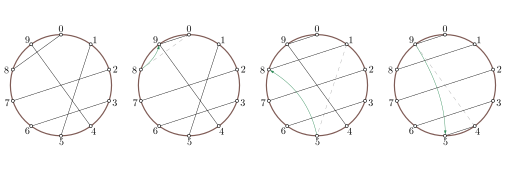
\includegraphics[width=\textwidth]{sample1}
\end{figure}

The figure below shows the initial state of the harp for samples 2, 3, and 4.

\begin{figure}
\centering
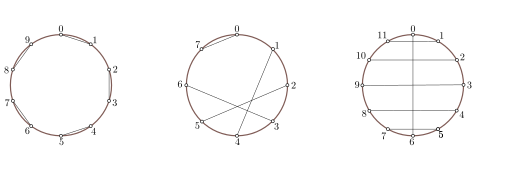
\includegraphics[width=\textwidth]{sample234}
\end{figure}

\begin{itemize}
\item The first sample satisfies the constraints of test groups 4 and 5.
\item The second sample satisfies the constraints of test groups 1, 3, 4, and 5.
\item The third sample satisfies the constraints of test groups 2, 4, and 5.
\item The fourth sample satisfies the constraints of test groups 3, 4, and 5.
\end{itemize}



